\documentclass{standalone}
\usepackage{tikz}
\usetikzlibrary{patterns}
\usetikzlibrary{positioning}
\usetikzlibrary{patterns, positioning}
\usetikzlibrary{shapes.misc}
\usepackage[outline]{contour}
\contourlength{1.5pt} 
\usepackage[sfdefault]{ClearSans}

\begin{document}
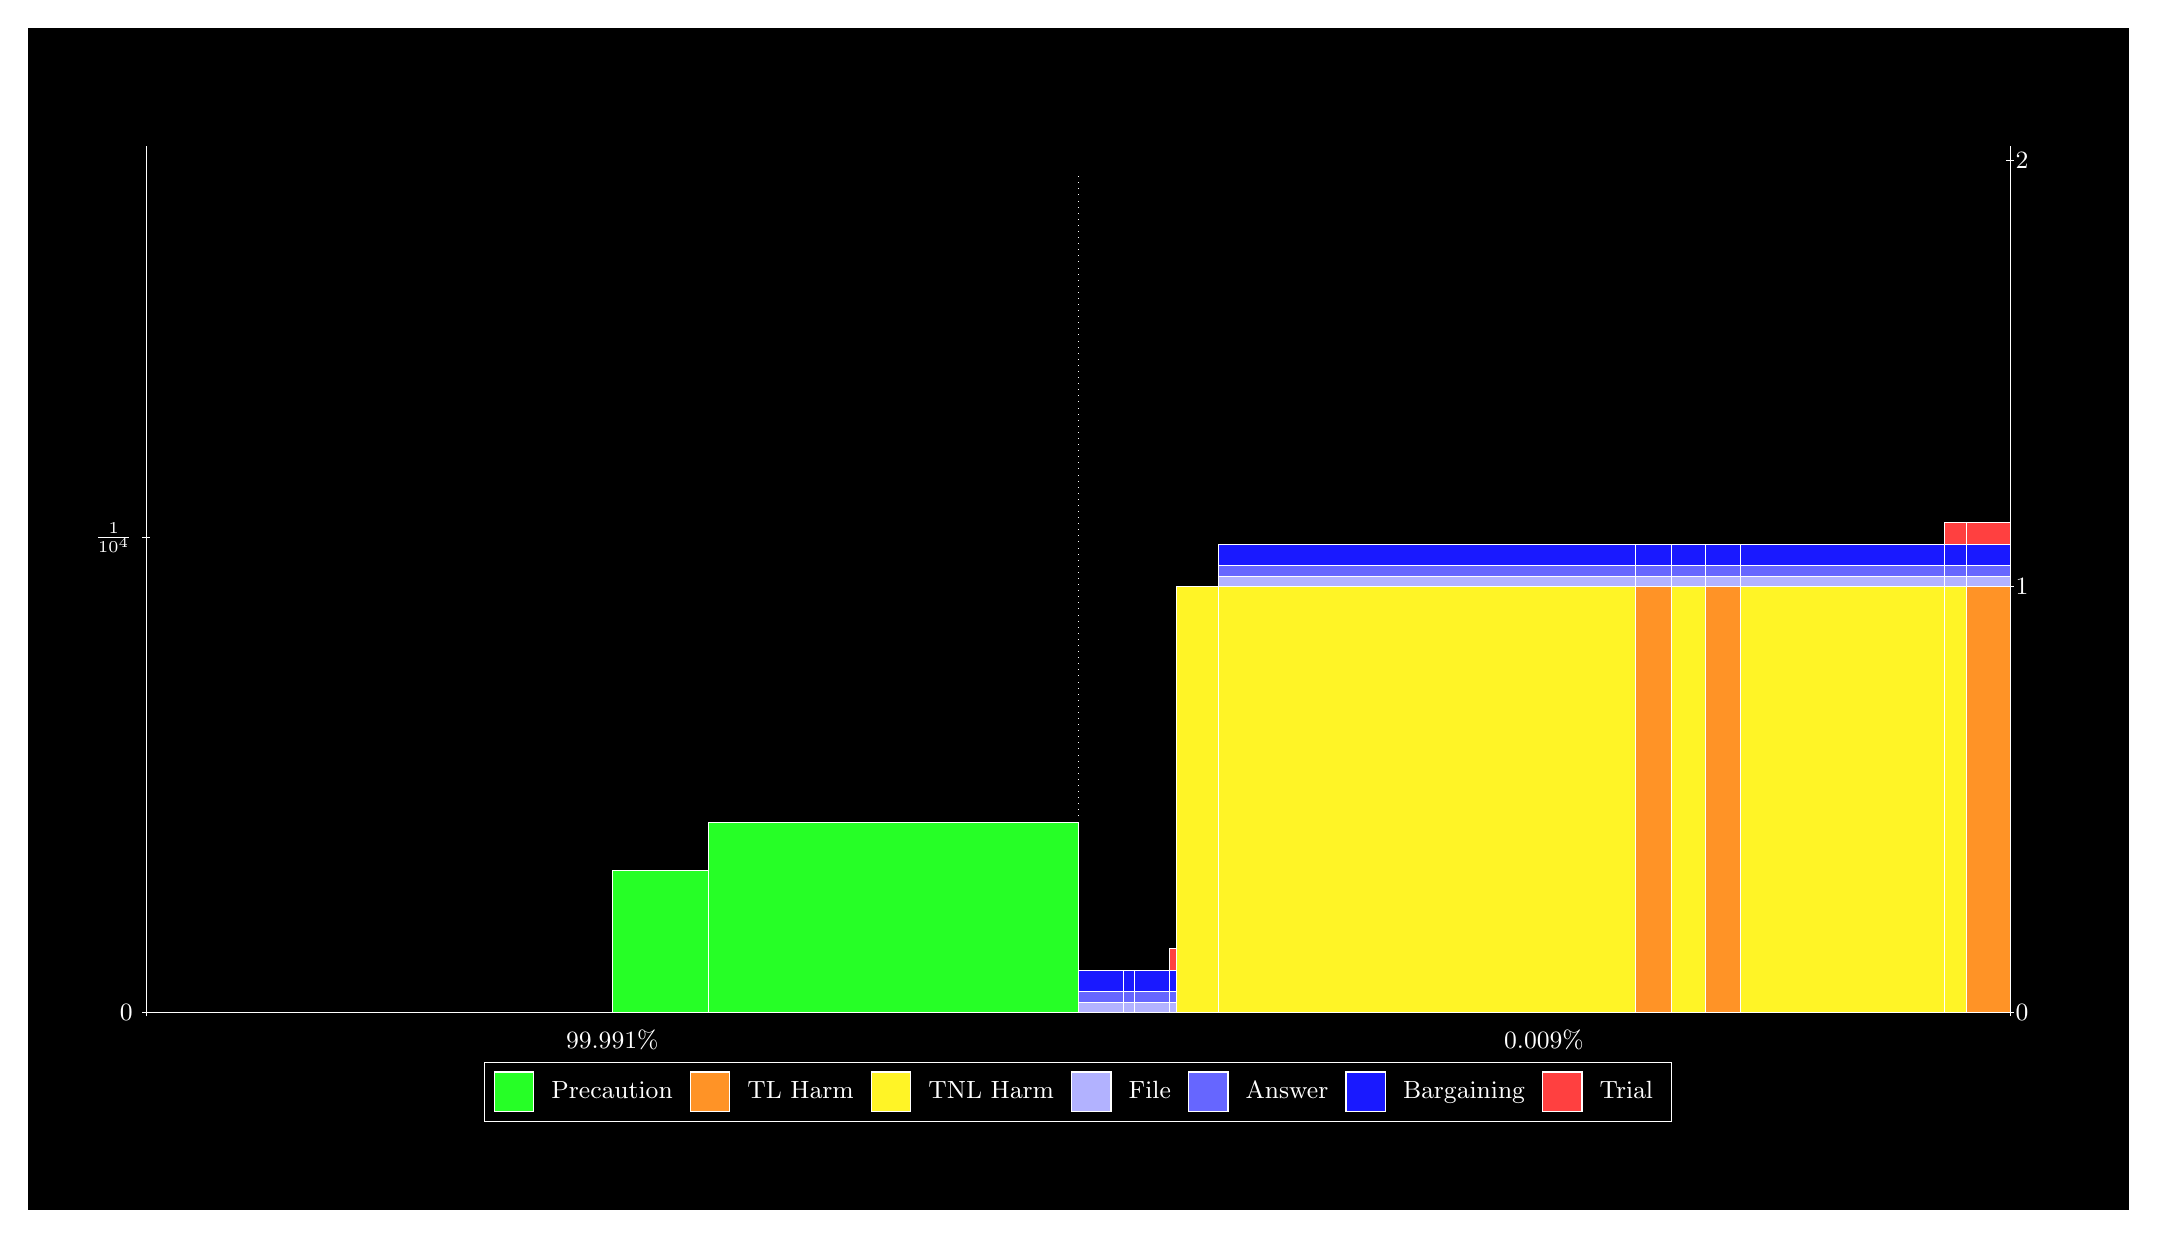
\begin{tikzpicture}
\draw[fill=black] (0,0) rectangle (26.667,15);
\draw[fill=green!85,draw=white,very thin] (7.4165,2.5) rectangle (8.6334,4.3088);
\draw[fill=green!85,draw=white,very thin] (8.6334,2.5) rectangle (13.333,4.9118);
\draw[fill=blue!30,draw=white,very thin] (13.333,2.5) rectangle (13.909,2.6352);
\draw[fill=blue!60,draw=white,very thin] (13.333,2.6352) rectangle (13.909,2.7704);
\draw[fill=blue!90,draw=white,very thin] (13.333,2.7704) rectangle (13.909,3.0409);
\draw[fill=green!85,draw=white,very thin] (13.909,2.5) rectangle (14.045,2.5002);
\draw[fill=blue!30,draw=white,very thin] (13.909,2.5002) rectangle (14.045,2.6354);
\draw[fill=blue!60,draw=white,very thin] (13.909,2.6354) rectangle (14.045,2.7706);
\draw[fill=blue!90,draw=white,very thin] (13.909,2.7706) rectangle (14.045,3.041);
\draw[fill=green!85,draw=white,very thin] (14.045,2.5) rectangle (14.493,2.5002);
\draw[fill=blue!30,draw=white,very thin] (14.045,2.5002) rectangle (14.493,2.6354);
\draw[fill=blue!60,draw=white,very thin] (14.045,2.6354) rectangle (14.493,2.7706);
\draw[fill=blue!90,draw=white,very thin] (14.045,2.7706) rectangle (14.493,3.0411);
\draw[fill=blue!30,draw=white,very thin] (14.493,2.5) rectangle (14.577,2.6352);
\draw[fill=blue!60,draw=white,very thin] (14.493,2.6352) rectangle (14.577,2.7704);
\draw[fill=blue!90,draw=white,very thin] (14.493,2.7704) rectangle (14.577,3.0409);
\draw[fill=red!75,draw=white,very thin] (14.493,3.0409) rectangle (14.577,3.3113);
\draw[fill=green!85,draw=white,very thin] (14.577,2.5) rectangle (15.112,2.5002);
\draw[fill=yellow!85,draw=white,very thin] (14.577,2.5002) rectangle (15.112,7.9088);
\draw[fill=yellow!85,draw=white,very thin] (15.112,2.5) rectangle (20.407,7.9086);
\draw[fill=blue!30,draw=white,very thin] (15.112,7.9086) rectangle (20.407,8.0438);
\draw[fill=blue!60,draw=white,very thin] (15.112,8.0438) rectangle (20.407,8.1791);
\draw[fill=blue!90,draw=white,very thin] (15.112,8.1791) rectangle (20.407,8.4495);
\draw[fill=orange!85,draw=white,very thin] (20.407,2.5) rectangle (20.871,7.9086);
\draw[fill=blue!30,draw=white,very thin] (20.407,7.9086) rectangle (20.871,8.0438);
\draw[fill=blue!60,draw=white,very thin] (20.407,8.0438) rectangle (20.871,8.1791);
\draw[fill=blue!90,draw=white,very thin] (20.407,8.1791) rectangle (20.871,8.4495);
\draw[fill=green!85,draw=white,very thin] (20.871,2.5) rectangle (21.303,2.5002);
\draw[fill=yellow!85,draw=white,very thin] (20.871,2.5002) rectangle (21.303,7.9088);
\draw[fill=blue!30,draw=white,very thin] (20.871,7.9088) rectangle (21.303,8.044);
\draw[fill=blue!60,draw=white,very thin] (20.871,8.044) rectangle (21.303,8.1792);
\draw[fill=blue!90,draw=white,very thin] (20.871,8.1792) rectangle (21.303,8.4496);
\draw[fill=green!85,draw=white,very thin] (21.303,2.5) rectangle (21.742,2.5002);
\draw[fill=orange!85,draw=white,very thin] (21.303,2.5002) rectangle (21.742,7.9088);
\draw[fill=blue!30,draw=white,very thin] (21.303,7.9088) rectangle (21.742,8.044);
\draw[fill=blue!60,draw=white,very thin] (21.303,8.044) rectangle (21.742,8.1792);
\draw[fill=blue!90,draw=white,very thin] (21.303,8.1792) rectangle (21.742,8.4496);
\draw[fill=green!85,draw=white,very thin] (21.742,2.5) rectangle (24.329,2.5002);
\draw[fill=yellow!85,draw=white,very thin] (21.742,2.5002) rectangle (24.329,7.9088);
\draw[fill=blue!30,draw=white,very thin] (21.742,7.9088) rectangle (24.329,8.0441);
\draw[fill=blue!60,draw=white,very thin] (21.742,8.0441) rectangle (24.329,8.1793);
\draw[fill=blue!90,draw=white,very thin] (21.742,8.1793) rectangle (24.329,8.4497);
\draw[fill=yellow!85,draw=white,very thin] (24.329,2.5) rectangle (24.612,7.9086);
\draw[fill=blue!30,draw=white,very thin] (24.329,7.9086) rectangle (24.612,8.0438);
\draw[fill=blue!60,draw=white,very thin] (24.329,8.0438) rectangle (24.612,8.1791);
\draw[fill=blue!90,draw=white,very thin] (24.329,8.1791) rectangle (24.612,8.4495);
\draw[fill=red!75,draw=white,very thin] (24.329,8.4495) rectangle (24.612,8.7199);
\draw[fill=orange!85,draw=white,very thin] (24.612,2.5) rectangle (25.167,7.9086);
\draw[fill=blue!30,draw=white,very thin] (24.612,7.9086) rectangle (25.167,8.0438);
\draw[fill=blue!60,draw=white,very thin] (24.612,8.0438) rectangle (25.167,8.1791);
\draw[fill=blue!90,draw=white,very thin] (24.612,8.1791) rectangle (25.167,8.4495);
\draw[fill=red!75,draw=white,very thin] (24.612,8.4495) rectangle (25.167,8.7199);
\draw[white,very thin] (1.5,2.5) -- (1.5,13.5);
\draw[white,very thin] (1.45,2.5) -- (1.55,2.5);
\node[font=\small,text=white, anchor=east] at (1.45, 2.5) {0};
\draw[white,very thin] (1.45,8.5295) -- (1.55,8.5295);
\node[font=\small,text=white, anchor=east] at (1.45, 8.5295) {$\frac{1}{10^{4}}$};

\draw[white,dotted,very thin] (13.333,2.83) -- (13.333,13.17);
\draw[white,very thin] (25.167,2.5) -- (25.167,13.5);
\draw[white,very thin] (25.117,2.5) -- (25.217,2.5);
\node[font=\small,text=white, anchor=west] at (25.117, 2.5) {0};
\draw[white,very thin] (25.117,7.9086) -- (25.217,7.9086);
\node[font=\small,text=white, anchor=west] at (25.117, 7.9086) {1};
\draw[white,very thin] (25.117,13.317) -- (25.217,13.317);
\node[font=\small,text=white, anchor=west] at (25.117, 13.317) {2};

\draw[white,very thin] (1.5,2.5) -- (25.167,2.5);
\draw[white,very thin] (1.5,2.45) -- (1.5,2.55);
\node[font=\small,text=white, anchor=north] at (1.5, 2.45) {};
\draw[white,very thin] (25.167,2.45) -- (25.167,2.55);
\node[font=\small,text=white, anchor=north] at (25.167, 2.45) {};

\node[font=\small,text=white,anchor=south] at (7.4167, 1.9) {99.991\%};
\node[font=\small,text=white,anchor=south] at (19.25, 1.9) {0.009\%};
\draw (13.3333,2.5) node (B) {};
\begin{scope}[align=center]
\matrix[scale=0.5,draw=white,below=0.5cm of B,nodes={draw},column sep=0.1cm]{
\node[rectangle,draw,minimum width=0.5cm,minimum height=0.5cm,fill=green!85]{}; & \node[draw=none,font=\small,text=white]{Precaution}; &
\node[rectangle,draw,minimum width=0.5cm,minimum height=0.5cm,fill=orange!85]{}; & \node[draw=none,font=\small,text=white]{TL Harm}; &
\node[rectangle,draw,minimum width=0.5cm,minimum height=0.5cm,fill=yellow!85]{}; & \node[draw=none,font=\small,text=white]{TNL Harm}; &
\node[rectangle,draw,minimum width=0.5cm,minimum height=0.5cm,fill=blue!30]{}; & \node[draw=none,font=\small,text=white]{File}; &
\node[rectangle,draw,minimum width=0.5cm,minimum height=0.5cm,fill=blue!60]{}; & \node[draw=none,font=\small,text=white]{Answer}; &
\node[rectangle,draw,minimum width=0.5cm,minimum height=0.5cm,fill=blue!90]{}; & \node[draw=none,font=\small,text=white]{Bargaining}; &
\node[rectangle,draw,minimum width=0.5cm,minimum height=0.5cm,fill=red!75]{}; & \node[draw=none,font=\small,text=white]{Trial}; \\\\
};\end{scope}

\end{tikzpicture}
\end{document}